\chapter{Inductors}
\label{chapInductors}

% Interesting link - http://info.ee.surrey.ac.uk/Workshop/advice/coils/terms.html http://info.ee.surrey.ac.uk/Workshop/advice/coils/Faraday/ http://pveducation.org/pvcdrom/2-properties-sunlight/photon-flux http://www.smpspowersupply.com/magnetic-unit-conversion.html https://www.physicsforums.com/threads/does-a-constant-electric-flux-produce-a-current.334458/ http://hyperphysics.phy-astr.gsu.edu/hbase/electric/pplate.html#c1  http://hyperphysics.phy-astr.gsu.edu/hbase/magnetic/magfie.html#c1  http://physics.info/inductance/
%

In this chapter, we will begin our study of \glossterm{inductors} and \glossterm{coils}.

\section{Inductors, Coils, and Magnetic Flux}

In Chapter~\ref{chapCapacitors}, we learned that capacitors stored charge by using an electric field.
We also learned that capacitors continued to hold their charge even after it was disconnected from the rest of the circuit.
We learned in Chapter~\ref{chapSound} that capacitors blocked DC signals but allowed AC signals to pass through.

\subsection{What is an Inductor?}
An inductor is kind of like the capacitor's evil twin.  
It behaves in some ways that remind us a lot of capacitors, but it is operating on a different aspect of electrical behavior.
Capacitors store charge and release it in response to voltage changes.
Inductors, instead, store \glossterm{magnetic flux} and release it in response to current changes.
Thus, capacitors tend to even out voltages, and inductors tend to even out currents.

\simplegraphicsfigure{The Symbol for an Inductor}{InductorSymbol}{0.125}

Figure~\ref{figInductorSymbol} shows what an inductor looks like in a schematic.
Inductors are non-polarized, so they can be wired in either direction.
The symbol loosely represents a coil of wire, because that is what inductors are essentially made of.

\subsection{What is magnetic flux?}
When current moves in a wire, it creates a very tiny magnetic field.
It's not large enough to pick up anything, but it is present.
Flux is the total amount of magnetism present in an inductor.
Since this is an engineering book, not a physics book, we won't spend a lot of time trying to come to grips with what flux is and how it works.
We will simply understand that it is the total size of the magnetic field of a component, and it is measured in Webers (Wb).
To get a feel for what a Weber is like, a small bar magnet has a flux of around $\frac{1}{1000}\mywb$.

As a side note, when we say that something is magnetic, we are usually not talking about the total flux of something, but of the \emph{density} of that flux---the amount of flux in an given area.
Flux density is measured in Teslas (one Tesla is $\frac{1\mywb}{1\textrm{ meter}^2}$), but we will not concern ourselves with Teslas or flux densities for this course.

\subsection{What is the difference between electric vs. magnetic fields}

Now, when we talked about capacitors, we talked a little bit about electric fields.
Electric fields and magnetic fields are related, but different.
An electric field is generated by a difference in charge between two surfaces.
Electric fields can exist even when no current is moving at all---there just has to be two differently-charged surfaces.
Basically, any charged object will induce a force on another charged object for a certain distance, and this is the electric field.

The magnetic field, however, only exists when a charge is moving.
When a charge is in motion, in addition to the electric field, it also creates a \emph{magnetic} field surrounding itself, going perpendicular to the wire.
This field also exhibits a force on charged objects within a small distance, but a much larger distance than the electric field.
Additionally, when the current in the wire slows down, the magnetic field will convert its own energy into current in the wire.

The size of a magnetic field within a single wire is very, very small, and can be ignored.
However, the strength of the magnetic field of a wire can be increased by wrapping (coiling) it around a cylindrical core.
This aligns the magnetic fields of the wires so that the fields can each be added together to produce a combined magnetic field.
Each turn around the core adds an additional bit to the magnetic field.
Devices based on this priciple are called coils or an \glossterm{inductors}.

When an inductor is first turned on, most of the current goes into creating the inductor's magnetic field.
Then, as the magnetic field is setting up, it allows more and more current to flow, until it hits a steady state.
Then, if the current flow reduces, the energy from the magnetic field gets transformed into current and goes out to try to make up the difference.

While a capacitor stores energy as a charge and releases it when there is a voltage change, an inductor stores energy as magnetic flux and releases it when there is a current change.
An inductor's inductance is measured using the \glossterm{Henry} (H).
The core equations of capacitors and inductors are related as well.
The defining equation of a capacitor is $Q = C\cdot V$, where $Q$ is the charge in the capacitor.
The defining equation of an inductor is just as simple:

\begin{equation}
\label{eqinductance}
\phi = L\cdot I
\end{equation}

In this equation, $\phi$ is the magnetic flux in the inductor (in Webers), $L$ is the inductance (in Henries), and $I$ is the current (in Amperes).
The \glossterm{Henry} is the primary unit of inductance, and has an abbreviation of $\myhy$.

\begin{exampleprob}
If I have a 50 microhenry inductor and have a constant current of 2 milliamps, how much magnetic flux is being stored?

\begin{align*}
\phi &= L\cdot I \\
L &= 50\myuhy = 0.00005\myhy \\
I &= 2\mymamp = 0.002\myamp
\phi &= 0.00005\cdot 0.002 \\
  &= 0.0000001\mywb = 0.1\myuwb
\end{align*}

Therefore, we have 0.0000001 Webers of flux, or 0.1 microwebers of flux.
\end{exampleprob}

Therefore, when a relatively constant amount of current flows, it is easy to calculate the amount of flux in the magnetic field.

\section{Induced Voltages}

Changes in the flux of a magnetic field induces voltages.
The amount of voltage induced depends on how fast the flux changes.
The induced voltage is essentially the change in the flux divided by the number of seconds that it took for the change to occur.
If the flux decreases, the energy is converted into voltage, which goes up.
If the flux increases, the energy was taken from the voltage, which goes down.
So, if there was a decrease of $10\mywb$ over the course of $2\mysec$ then the amount of voltage induced would be $\frac{10\mywb}{2\mysec} = 5\myvolt$.

The formal statement of this is known as Lenz's law.  It is given as follows:

\begin{equation}
\label{eqlenz}
V_{\textrm{average}} = -\frac{\textrm{change in }\phi}{\textrm{change in time}}
\end{equation}

The average voltage produced by the change in a magnetic field over a given time period is the same as the amount of flux that was reduced by the field divided by the same time period.

Now, the amount of flux in the inductor will change with the current, as indicated by Equation~\ref{eqinductance}.
When the current decreases, it will cause the flux to be converted into voltage.
When the current increases, it will add more flux into the magnetic field, using up voltage.

When the amount of flux changes, it creates a voltage.
The amount of flux change (in Webers) divided by the amount of time it took to change (in seconds) will yield the voltage produced by the change.
Therefore, when the current drops, the flux will be converted to voltage.
If we add in voltage, it will also increase the current.

\section{Resisting Changes in Current}

Ultimately, what an inductor is doing is resisting changes in current.
When the current goes up, the current is first used to construct the magnetic field, and therefore it takes some time to allow the full amount of current through.
When the current goes down, the flux of the magnetic field decreases, which gets converted back to voltage, which induces more current.

The inductor, with regards to current, is the opposite of the capacitor.
With direct current, the capacitor, when first connected to the circuit, acts as a short circuit---the current basically flows right through until the capacitor starts to fill up.
When the capacitor is full, then it acts like an open circuit---blocking any more current from flowing.

The inductor is the opposite.
When first connected to the circuit, the inductor acts like an open circuit---the current is basically being used to construct the magnetic field.
As the magnetic field strength increases, more and more current is allowed to flow.
Once the magnetic field flux matches what it should be for the given current, the current flows freely, as if the inductor were not even there, like a short circuit.

In summary, we can say that a capacitor acts as an open circuit for sustained DC current and as a short circuit for alternating current.
The inductor acts as a short circuit for sustained DC current and as an open circuit for alternating current.

\section{Analogy from Mechanics}

If you are into mechanics, you can think of an inductor as a flywheel.
Flywheels store mechanical energy into the motion of a large or heavy wheel.
It takes energy to get the wheel spinning, but once it is spinning, the wheel itself can continue to drive the mechanism.
The wheel is used to even out the drive of the other components of the mechanism.

For instance, an engine driven by pistons will have somewhat irregular motion, because the force of the pistons is not constant through their motion.
However, attaching a flywheel will even out the energy output. 
When the pistons are delivering more power, most of the excess will be going to the flywheel, and when the pistons are delivering less power, the mechanism can be driven by the force of the flywheel.

\section{Uses of Inductors}

Inductors are used in a very wide variety of applications---much more so than capacitors.
Capacitors are used primarily for their effects \emph{within} electronic circuits---filtering noise, blocking DC current, coupling DC-biased circuits, etc.
However, the electric field created on the plates of the capacitor is fairly useless on its own because the field fades so quickly with distance.
Inductors are used for similar things as capacitors within circuits (their operation being largely the counterpart of what a capacitor would do), but additionally, the magnetic field of the inductor has innumerable uses because its effects are stronger further away.
These uses include:

\begin{itemize}
\item Inductors are used to make \glossterm{electromagnets}, for picking up and setting down large objects.  
\item Inductors are used to make \glossterm{transformers}, which use the magnetic field in one inductor to generate a current in another inductor.
\item Inductors are used to make motors, where the electromagnetic coils are used to turn a shaft.
\item Inductors are used to make speakers, which use the magnetic field to move the speaker diaphragm back and forth.
\item Inductors are used to make relays, which use the magnetic field to open and close switches.
\end{itemize}

These are just some of the uses of inductors.  
In short, the magnetic field created by the inductor is what allows many of the interfaces between electronic devices and the real world.

\section{Inductive Kick}

One important thing to keep in mind when using inductors is the concept of inductive kick.
Lenz's law (Equation~\ref{eqlenz}) shows that decreases in the magnetic flux will induce a voltage.  
Since the magnetic flux is divided by time to get the voltage, that means that a shorter timespan will generate a larger voltage.
Thus, a sudden decrease in magnetic flux will cause a voltage spike.

But what controls the flux?
If you go back to Equation~\ref{eqinductance}, we can see that a decrease in current will decrease the magnetic flux.
Therefore, a sudden decrease in current will cause a sudden decrease in the magnetic flux which will then cause a large voltage spike within the inductor itself.
This spike is known as an \glossterm{inductive kick} and can damage nearby electronic components.
To avoid an inductive kick, a \glossterm{flyback diode}, also called a \glossterm{protection diode} or a \glossterm{snubber diode}, can be used.

A flyback diode is a regular diode (\emph{not} a Zener diode) wired backwards across the terminals of an inductor.
Under normal operation the diode won't conduct.
However, when the diode is shut off, it provides a safe path for the generated voltage to pass through (back through the other side of the inductor), and allows the inductor to bleed off voltage in a much more controlled manner.

\simplepdffigure{A Snubber Diode}{SnubberDiode}{0.25}

Figure~\ref{figSnubberDiode} shows how this is wired up.  
As you can see, under normal operation, the current flows in the direction of the arrow.
Since the left-hand side is more positive than the right-hand side, no current can flow through the diode.
However, when the current is shut off, the right-hand side becomes more positive very quickly, and the diode feeds the excess current back through the inductor to allow the extra energy dissipate more slowly.

You might be wondering why the voltage doesn't just shift back to the left side on its own once the right-hand side is more positive.
The answer is that the magnetic field that is generating the voltage is itself directionalized within the inductor.  The field's movement is such that it is essentially pushing current to the right (which is why a voltage is being produced).
Therefore, the flyback diode carries this excess voltage back to the left-hand side of the diode.

Flyback diodes are used with all sorts of inductors (motors, electromagnets, etc.) anywhere where there are components that could be damaged by an inductive kick.
For basic applications, nearly any type of diode will work for a flyback diode.
However, diodes differ in their speed in reacting to voltage changes.
In some circuits, the speed that a diode reacts to changes in voltage can be important.

\reviewsection

In this chapter, we learned:

\begin{enumerate}
\item Inductors are electronic components that are made of winding wire around a core which allows them to store charge in their magnetic fields.
\item The strength of a magnetic field is the magnetic flux and is measured in Webers (Wb).
\item While an \emph{electric} field is made from the \emph{presence} of charges, the \emph{magnetic} field is made from the \emph{movement} of charges (i.e., the current).
\item When the current going into an inductor increases, the extra current is first used to build up the flux of the magnetic field before achieving a new steady state.
\item When the current going into an inductor decreases, the flux of the magnetic field is converted into a voltage, which increases the output current, resisting the change in current.
\item Inductors oppose changes in current.  They act as resistors to AC current and as short circuits to DC current.
\item An inductor can be thought of similar to a flywheel in mechanics, which stores energy in a rotating wheel.
\item Inductors are useful because not only do they have interesting electric properties, their magnetic field also allows them to interface into the real world because magnetic field effects have a much longer reach than electric field effects.
\item When current to an inductor is suddenly shut off, it creates a large voltage, known as an inductive kick.
\item A snubber diode is used to mitigate against the negative effects of an inductive kick.
\end{enumerate}

\applysection


\begin{enumerate}
\item 
\question{If I want a circuit to block DC current but allow AC current, should I use an inductor or a capacitor?}
\solution{Capacitor}
\explanation{Capacitors allow AC current but block DC current.}
\item 
\question{If I want a circuit to allow DC current but block AC current, should I use an inductor or a capacitor?}
\solution{Inductor}
\explanation{Inductors allow DC current but block AC current.}
\item 
\question{Why are inductors used so much in systems that interact with the outside world?}
\solution{Inductors create a magnetic field which can be used to move other components.}
\item 
\question{Why does inductive kick happen?}
\solution{In an inductor, the magnetic field is maintained through current flow through the inductor.  If the current decreases, the magnetic field cannot be maintained, and the flux is converted to a voltage.  A sudden decrease in current will cause an equally sudden build-up in voltage.  This is the inductive kick.}
\item 
\question{Draw a schematic of an inductor where the positive side of the inductor has a switch and the negative side is connected to an LED and a resistor.  Add in a snubber diode to protect the LED from the effect of turning off the switch.}
\solution{\newline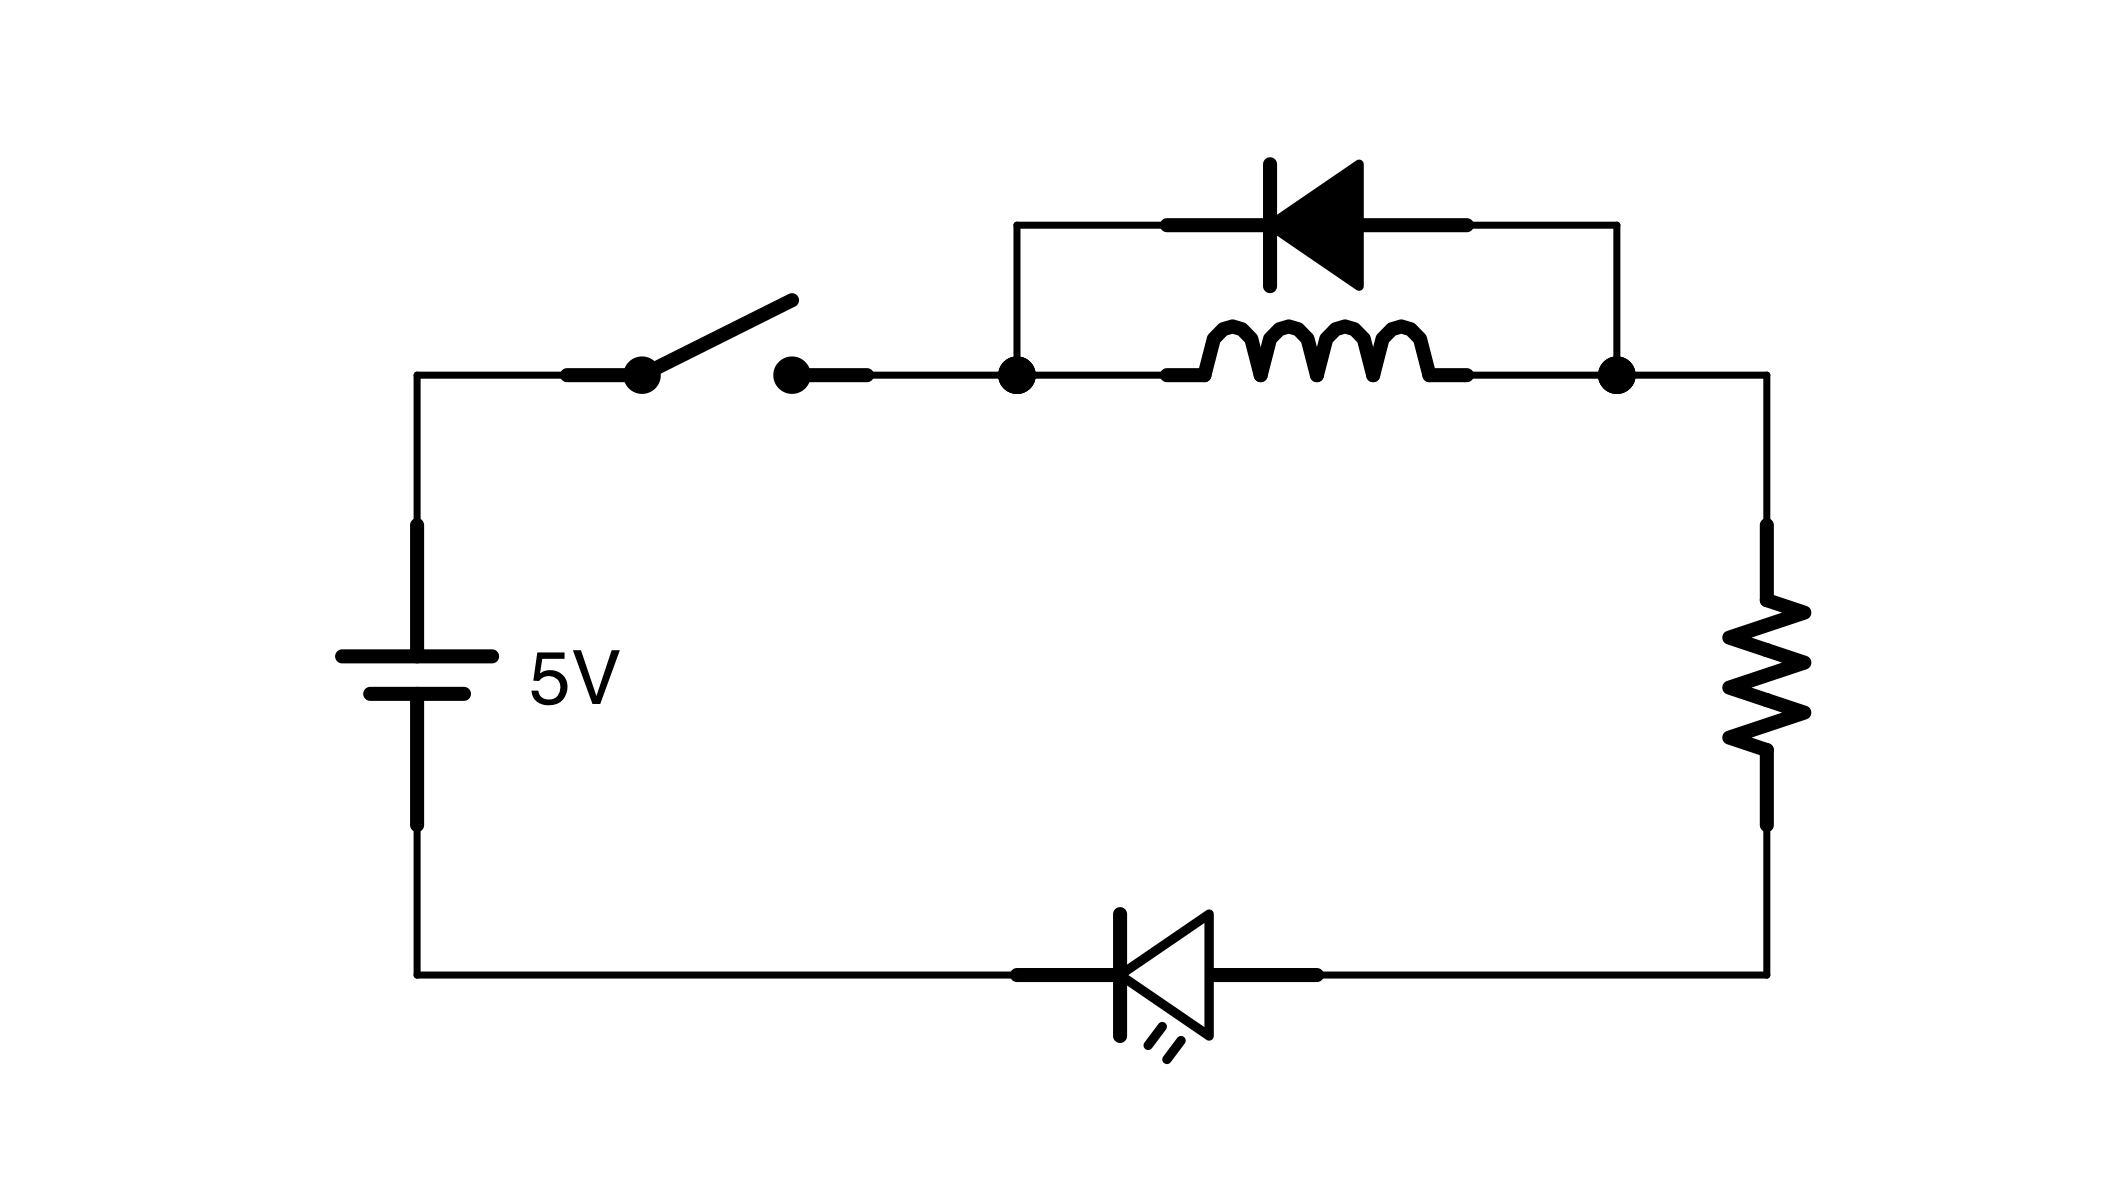
\includegraphics[width=0.7\columnwidth]{SolutionSnubberDiode.png}}
\item
\question{What is the purpose of the snubber diode?}
\solution{The snubber diode reduces the effect of the inductive kick by giving the current a pathway back through the inductor.
This allows generated voltages/currents to be bled off slowly throught the inductor itself.}
\item 
\question{If I have an inductor that is $5\myhy$ and has a steady current going through it of $2\myamp$, what is the size of the magnetic flux in the inductor's magnetic field?}
\solution{$10$ webers}
\explanation{The equation governing the behavior of an inductor is given by Equation~\ref{eqinductance}, $\phi = L \cdot I$, where $L$ is given in henries and $I$ is in amperes.
Therefore, since the units match, we can calculate as follows:
\begin{align*}
\phi &= L \cdot I \\
 &= 5 \cdot 2 \\
 &= 10
\end{align*}
Therefore, the inductor is holding $10$ webers of flux.
}
\item 
\question{If I have an inductor that is $7\myuhy$ and has a steady current going through it of $3\mymamp$, what is the size of the magnetic flux in the inductor's magnetic field?}
\solution{$0.000000021$ webers}
\explanation{The equation for flux is $\phi = L \cdot I$, where $L$  is in henries and $I$ is in amperes.
Therefore, we need to convert into proper units to use the equation.
Since $1\myuhy = 0.000001\myhy$, $7\myuhy = 0.000007\myhy$.
Since $1\mymamp = 0.001\myamp$, $3\mymamp = 0.003\myamp$.
Therefore, the equation becomes:
\begin{align*}
\phi &= L \cdot I \\
 &= 0.000007 \cdot 0.03 \\
 &=0.000000021
\end{align*}
Therefore, the magnetic field has a flux of $0.000000021$ webers.
}
\item 
\question{If I have a $4\myhy$ inductor with $0.3\mywb$ of flux in its magnetic field, how much current is flowing through it?}
\solution{$0.075\myamp$ or $75\mymamp$}
\explanation{We will solve this problem by rearranging Equation~\ref{eqinductance} to solve for $I$:
\begin{align*}
\phi &= L \cdot I \\
I &= \frac{\phi}{L}
\end{align*}
Since the units are already correct, I can now just substitute and solve:
\begin{align*}
I &= \frac{\phi}{L} \\
 &= \frac{0.3}{4} \\
 &= 0.075
\end{align*}
Therefore, the current is $0.075\myamp$ or $75\mymamp$.
}
\item 
\question{If an inductor's magnetic field has $5\mywb$ of flux and it decreases to $3\mywb$ of flux over $2\mysec$, what is the average voltage produced over that timeframe?}
\solution{}
\explanation{Questions involving the \emph{change} of voltage and flux utilize Equation~\ref{eqlenz}, which states:
\begin{align*}
V_{\textrm{average}} = -\frac{\textrm{change in }\phi}{\textrm{change in time}}
\end{align*}
Since we start with $5\mywb$ of flux and end with $3\mywb$, therefore, we changed by $-2\mywb$.
Since this occurred across $2\mysec$, the resulting formula would be:
\begin{align*}
V_{\textrm{average}} &= -\frac{-2}{2} \\
  &= 1
\end{align*}
Therefore, the average voltage produced for that time period is $1\myvolt$.
}
\item 
\question{If an inductor's magnetic field has $1\myuwb$ of flux and it increases to $2\myuwb$ of flux over $0.4\mysec$, what is the average voltage produced over that timeframe?}
\solution{}
\explanation{Questions involving the \emph{change} of voltage and flux utilize Equation~\ref{eqlenz}.  To use this equation, first we have to convert units.
The standard conversion is $1\myuwb = 0.000001\mywb$.
Therefore, the equation becomes:
\begin{align*}
V_{\textrm{average}} &= -\frac{\textrm{change in }\phi}{\textrm{change in time}} \\
 &= -\frac{0.000001}{0.4} \\
 &= -0.0000025
\end{align*}
Therefore, the inductor will produce a negative voltage, averaging $-0.0000025\myvolt$ for the duration of the $0.4\mysec$.
}
\item 
\question{If the current flowing through a $3\myhy$ inductor drops from $7\mymamp$ to $1\mymamp$ over a period of $0.01\mysec$, what is the average voltage produced over that time period?}
\solution{$1.8\myvolt$}
\explanation{To solve this, you will need \emph{both} Equation~\ref{eqinductance} and Equation~\ref{eqlenz}.
Equation~\ref{eqlenz} requires a starting and an ending flux. 
However, we are not given the starting and ending flux, but rather the starting and ending current.
Equation~\ref{eqinductance} tells us how to relate current to the amount of flux.

First, we need to convert our units.
$7\mymamp = 0.007\myamp$ and $1\mymamp = 0.001\myamp$.
Let's begin by solving for the starting flux:
\begin{align*}
\phi &= L \cdot I \\
 &= 3 \cdot 0.007 \\
 &= 0.021
\end{align*}
So the starting flux is $0.021\mywb$.

Next, let's solve for the final flux:
\begin{align*}
\phi &= L \cdot I \\
 &= 3 \cdot 0.001 \\
 &= 0.003
\end{align*}
So, the final flux is $0.003\mywb$.
This means that the change in flux was $-0.018\mywb$ across $0.01\mysec$.
Therefore, the average voltage over that period can be found using Equation~\ref{eqlenz}:
\begin{align*}
V_{\textrm{average}} &= -\frac{\textrm{change in }\phi}{\textrm{change in time}} \\
 &= -\frac{-0.018}{0.01} \\
 &= 1.8
\end{align*}
Therefore, the average voltage produced by the decrease in current over that time period is $1.8\myvolt$.
}
\end{enumerate}

